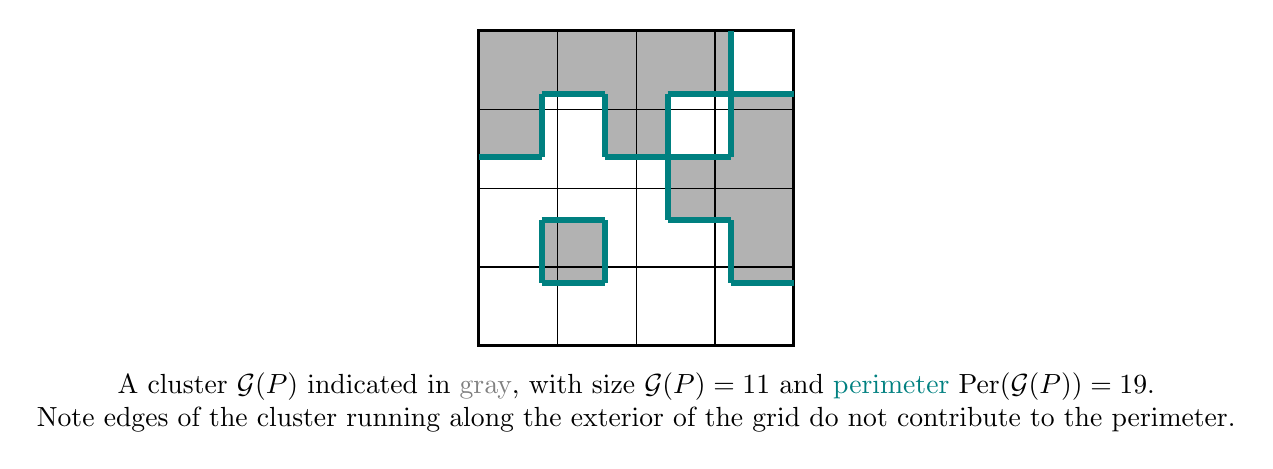
\begin{tikzpicture}[x=8mm,y=8mm,line cap=butt]

%--- 1) Fill the cluster cells (5x5 grid, origin at bottom-left) ---
% Gray cells: top row (1–4), second row (1,3,5), third row (4,5), fourth row (2,5)
\foreach \x/\y in {0/4,1/4,2/4,3/4, 0/3,2/3,4/3, 3/2,4/2, 1/1,4/1} {
  \fill[gray!60] (\x,\y) rectangle ++(1,1);
}

%--- 2) Draw grid (thin) and outer border (thick) ---
\draw[line width=0.5pt] (0,0) grid (5,5);
\draw[line width=1.2pt] (0,0) rectangle (5,5);

%--- 3) Draw the perimeter segments (interior edges only) ---
\begin{scope}[draw=teal,line width=2.2pt]
  % Vertical interior edges
  \draw (1,3)--(1,4);
  \draw (1,1)--(1,2);
  \draw (2,3)--(2,4);
  \draw (2,1)--(2,2);
  \draw (3,3)--(3,4);
  \draw (3,2)--(3,3);
  \draw (4,4)--(4,5);
  \draw (4,3)--(4,4);
  \draw (4,1)--(4,2);

  % Horizontal interior edges
  \draw (1,4)--(2,4);
  \draw (3,4)--(4,4);
  \draw (4,4)--(5,4);

  \draw (0,3)--(1,3);
  \draw (2,3)--(3,3);
  \draw (3,3)--(4,3);

  \draw (1,2)--(2,2);
  \draw (3,2)--(4,2);

  \draw (1,1)--(2,1);
  \draw (4,1)--(5,1);
\end{scope}

%--- 4) Caption / description ---
\node[align=center] at (2.5,-0.9)
{A cluster $\mathcal{G}(P)$ indicated in \textcolor{gray}{gray}, with size
$\lvert\mathcal{G}(P)\rvert=11$ and \textcolor{teal}{perimeter}
$\mathrm{Per}(\mathcal{G}(P))=19$.\\
Note edges of the cluster running along the exterior of the grid do not contribute to the perimeter.};

\end{tikzpicture}